%!TeX program = xelatex
\documentclass[12pt,hyperref,a4paper,UTF8]{ctexart}
\usepackage{HDUReport}
\usepackage{listings}
\usepackage{xcolor}

\usepackage{setspace}
\setstretch{1.5} % 设置全局行距为1.5倍

\usepackage{enumitem} % 载入enumitem包以便自定义列表环境
\setlist[itemize]{itemsep=0pt, parsep=0pt} % 设置itemize环境的项目间距和段落间距

\setmainfont{Times New Roman} % 英文正文为Times New Roman


% 自定义 Bash 脚本代码样式
\lstdefinelanguage{bash}{
    keywords={if, else, fi, for, while, do, done, exit, return, local, then, function},
    keywordstyle=\color{blue}\bfseries,
    ndkeywords={echo, printf, cat, grep, awk, sed, tr, chmod, cd, pwd, ls, mv, cp, rm},
    ndkeywordstyle=\color{teal}\bfseries,
    identifierstyle=\color{black},
    sensitive=true,
    comment=[l]{\#},
    commentstyle=\color{gray}\ttfamily,
    stringstyle=\color{red}\ttfamily,
    morestring=[b]",
    morestring=[b]',
}

\lstset{
    language=bash,
    basicstyle=\ttfamily\small, % 设置代码字体和大小
    numbers=left, % 显示行号
    numberstyle=\tiny\color{gray}, % 行号样式
    stepnumber=1, % 行号递增
    numbersep=5pt, % 行号与代码的间距
    backgroundcolor=\color{white}, % 背景颜色
    frame=single, % 代码框样式
    breaklines=true, % 自动换行
    captionpos=b, % 标题位置
    tabsize=4, % Tab 宽度
    showspaces=false, % 不显示空格
    showstringspaces=false, % 不显示字符串中的空格
}

%封面页设置
{   
    %标题
    \title{ 
        \vspace{1cm}
        \heiti \Huge \textbf{Linux系统及应用作业报告} \par
        \vspace{1cm} 
        \heiti \Large {\underline{作业5:使用Shell命令实现一种简单加密}   } 
        \vspace{3cm}
    
    }

    \author{
        \vspace{0.5cm}
        \kaishu\Large 学院\ \dlmu[9cm]{卓越学院} \\ %学院
        \vspace{0.5cm}
        \kaishu\Large 学号\ \dlmu[9cm]{23040447} \\ %班级
        \vspace{0.5cm}
        \kaishu\Large 姓名\ \dlmu[9cm]{陈文轩} \qquad  \\ %学号
        \vspace{0.5cm}
        \kaishu\Large 专业\ \dlmu[9cm]{智能硬件与系统(电子信息工程)} \qquad \\ %姓名 
    }
        
    \date{\today} % 默认为今天的日期,可以注释掉不显示日期
}
%%------------------------document环境开始------------------------%%
\begin{document}

%%-----------------------封面--------------------%%
\cover
\thispagestyle{empty} % 首页不显示页码
%%------------------摘要-------------%%
%\newpage
%\begin{abstract}




%\end{abstract}

%\thispagestyle{empty} % 首页不显示页码

%%--------------------------目录页------------------------%%
% \newpage
% \tableofcontents
% \thispagestyle{empty} % 目录不显示页码

%%------------------------正文页从这里开始-------------------%
\newpage
\setcounter{page}{1} % 让页码从正文开始编号

%%可选择这里也放一个标题
%\begin{center}
%    \title{ \Huge \textbf{{标题}}}
%\end{center}

\section{解密密文与明文推导}

\subsection{问题分析}
已知密文为:
\begin{itemize}
    \item Yfqp nx hmjfu
    \item Bmjwj ymjwj nx f xmjqg ymjwj nx f bfd
    \item Xmtb rj ymj htij
\end{itemize}
加密方法为:每个英文字母替换为ASCII字母表中后移 \( n \) 个位置的字母,大小写区分,标点符号和空格不变。例如,\( n=1 \) 时,A 变为 B,Z 变为 A。目标是确定 \( n \) 值并解密明文。

\subsection{解密思路}
以第一段密文 “Yfap nx hmjfu” 为例,假设其明文为常见英文单词,尝试推导 \( n \)。注意到密文中有 “nx”,可能对应明文中的常见双字母词如 “is”。若 “nx” 解密为 “is”,则:
- n 解密为 i:n(ASCII 110)向前 \( n \) 个位置为 i(ASCII 105),则 \( 110 - n = 105 \),\( n = 5 \)。
- x 解密为 s:x(ASCII 120)向前 \( n \) 个位置为 s(ASCII 115),同样 \( 120 - n = 115 \),\( n = 5 \)。



\subsection{解密结果}
- \( n \) 值为 5。
- 明文为:
\begin{itemize}
    \item Talk is cheap
    \item Where there is a shell there is a way
    \item Show me the code
\end{itemize}

\section{脚本编写}

\subsection{}

以下是实现加密和解密功能的 Shell 脚本代码:

\begin{lstlisting}[language=bash, caption={加密与解密脚本}, label={lst:encrypt_script}]
#!/bin/bash

# Function to encrypt text
encrypt() {
    local text="$1"
    local shift="$2"
    local result=""
    for ((i = 0; i < ${#text}; i++)); do
        char="${text:i:1}"
        if [[ "$char" =~ [A-Z] ]]; then
            # Uppercase letters
            result+=$(printf "\\$(printf '%03o' $(( ( $(printf '%d' "'$char") - 65 + shift ) % 26 + 65 )))")
        elif [[ "$char" =~ [a-z] ]]; then
            # Lowercase letters
            result+=$(printf "\\$(printf '%03o' $(( ( $(printf '%d' "'$char") - 97 + shift ) % 26 + 97 )))")
        else
            # Non-alphabetic characters (unchanged)
            result+="$char"
        fi
    done
    echo "$result"
}

# Function to decrypt text
decrypt() {
    local text="$1"
    local shift="$2"
    local result=""
    for ((i = 0; i < ${#text}; i++)); do
        char="${text:i:1}"
        if [[ "$char" =~ [A-Z] ]]; then
            # Uppercase letters
            result+=$(printf "\\$(printf '%03o' $(( ( $(printf '%d' "'$char") - 65 - shift + 26 ) % 26 + 65 )))")
        elif [[ "$char" =~ [a-z] ]]; then
            # Lowercase letters
            result+=$(printf "\\$(printf '%03o' $(( ( $(printf '%d' "'$char") - 97 - shift + 26 ) % 26 + 97 )))")
        else
            # Non-alphabetic characters (unchanged)
            result+="$char"
        fi
    done
    echo "$result"
}

# Parse command-line arguments
while [[ $# -gt 0 ]]; do
    case "$1" in
    -s)
        input_string="$2"
        shift 2
        ;;
    -k)
        shift_value="$2"
        shift 2
        ;;
    -if)
        input_file="$2"
        shift 2
        ;;
    -of)
        output_file="$2"
        shift 2
        ;;
    -d)
        mode="decrypt"
        shift
        ;;
    *)
        echo "Invalid option: $1"
        exit 1
        ;;
    esac
done

# Validate shift value
if [[ -z "$shift_value" || ! "$shift_value" =~ ^[0-9]+$ ]]; then
    echo "Error: Shift value (-k) must be a positive integer."
    exit 1
fi

# Perform encryption or decryption
if [[ -n "$input_string" ]]; then
    if [[ "$mode" == "decrypt" ]]; then
        result=$(decrypt "$input_string" "$shift_value")
    else
        result=$(encrypt "$input_string" "$shift_value")
    fi
    echo "$result"
elif [[ -n "$input_file" ]]; then
    if [[ ! -f "$input_file" ]]; then
        echo "Error: Input file not found."
        exit 1
    fi
    input_content=$(cat "$input_file")
    if [[ "$mode" == "decrypt" ]]; then
        result=$(decrypt "$input_content" "$shift_value")
    else
        result=$(encrypt "$input_content" "$shift_value")
    fi
    if [[ -n "$output_file" ]]; then
        echo "$result" >"$output_file"
    else
        echo "$result"
    fi
else
    echo "Error: No input provided. Use -s for string input or -if for file input."
    exit 1
fi
\end{lstlisting}


\subsection{代码解释}

上述脚本实现了一个简单的加密和解密工具,基于凯撒密码(Caesar Cipher)的原理。以下是脚本的主要功能和实现细节:

\begin{itemize}
    \item \textbf{加密函数(encrypt)}:
    \begin{itemize}
        \item 输入一个字符串和一个位移值(shift)。
        \item 遍历字符串中的每个字符:
        \begin{itemize}
            \item 如果是大写字母(A-Z),通过公式 \((\text{ASCII值} - 65 + \text{shift}) \% 26 + 65\) 计算加密后的字符。
            \item 如果是小写字母(a-z),通过公式 \((\text{ASCII值} - 97 + \text{shift}) \% 26 + 97\) 计算加密后的字符。
            \item 非字母字符(如空格、标点符号)保持不变。
        \end{itemize}
        \item 最终返回加密后的字符串。
    \end{itemize}

    \item \textbf{解密函数(decrypt)}:
    \begin{itemize}
        \item 输入一个字符串和一个位移值(shift)。
        \item 遍历字符串中的每个字符:
        \begin{itemize}
            \item 如果是大写字母(A-Z),通过公式 \((\text{ASCII值} - 65 - \text{shift} + 26) \% 26 + 65\) 计算解密后的字符。
            \item 如果是小写字母(a-z),通过公式 \((\text{ASCII值} - 97 - \text{shift} + 26) \% 26 + 97\) 计算解密后的字符。
            \item 非字母字符保持不变。
        \end{itemize}
        \item 最终返回解密后的字符串。
    \end{itemize}

    \item \textbf{命令行参数解析}:
    \begin{itemize}
        \item 使用 \texttt{while} 循环和 \texttt{case} 语句解析命令行参数。
        \item 支持的参数包括:
        \begin{itemize}
            \item \texttt{-s}:指定输入字符串。
            \item \texttt{-k}:指定加密/解密的位移值。
            \item \texttt{-if}:指定输入文件。
            \item \texttt{-of}:指定输出文件。
            \item \texttt{-d}:指定解密模式(如果不加 \texttt{-d},默认为加密模式)。
        \end{itemize}
    \end{itemize}

    \item \textbf{加密/解密逻辑}:
    \begin{itemize}
        \item 如果提供了字符串输入(\texttt{-s}),直接调用加密或解密函数处理字符串。
        \item 如果提供了文件输入(\texttt{-if}),读取文件内容并调用加密或解密函数处理。
        \item 如果指定了输出文件(\texttt{-of}),将结果写入文件;否则直接输出到终端。
    \end{itemize}

    \item \textbf{错误处理}:
    \begin{itemize}
        \item 如果未提供必要的参数(如 \texttt{-s} 或 \texttt{-if}),脚本会提示错误并退出。
        \item 如果位移值(\texttt{-k})不是正整数,脚本会提示错误并退出。
        \item 如果输入文件不存在,脚本会提示错误并退出。
    \end{itemize}
\end{itemize}

\subsection{脚本测试}



\begin{figure} % [H] 表示强制当前位置插入
        \centering
        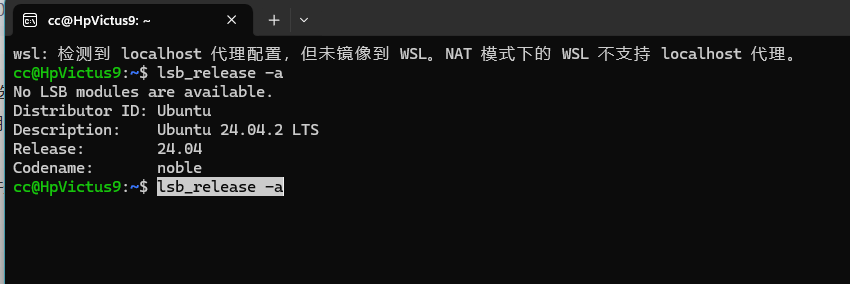
\includegraphics[width=0.9\textwidth]{figures/201.png} % 调整宽度为文本宽度的 80%
        \caption{WSL指令测试结果} %图片标题
        \label{fig:example} % 图片标签,用于引用
\end{figure}


\begin{figure} % [H] 表示强制当前位置插入
        \centering
        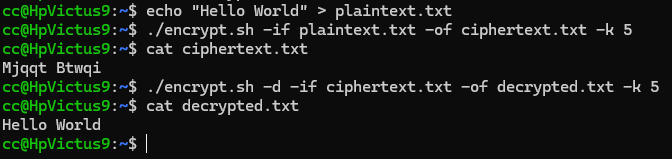
\includegraphics[width=0.9\textwidth]{figures/202.png} % 调整宽度为文本宽度的 80%
        \caption{WSL文件测试结果} %图片标题
        \label{fig:example} % 图片标签,用于引用
\end{figure}


\end{document}